\section{Resisitive switch design}
\label{sec:resisitive_switch_design}
This chapter will show the theoretical concepts and propose a design of a cantilever based micro-switch.
Trade-offs and important parameters will be explained.
Also all simplifications are described here.

\subsection{Contact}
\label{sec:contact}
Optimized contact pads have serious constraints on geometry, materials, contact force and release force. 
Due to the small scope of this project the contact pads were not further studied and were defined as being of a simple rectangular shape.
The material was chosen to be gold for it's good electric and mechanical properties. 

A choice was made between two designs.
The first possibility was to use a cantilever with a single contact point, so that the current would flow through the cantilever itself. %image
The second possibility was to use a cantilever with a simple golden surface, that would connect two fixed contact points to one another. %image
The second design was chosen to guarantee a small lenght of the contact element and therefore to reduce it's resistance and power consumption.
Also the mechanical properties of the cantilever don't get influenced that heavily by the second choice and therefore enables the design, of all but the tip of the cantilever, to focus on the actuation and guidance functionality of the structure.
The disadvantage of this design choice is a minimum required width, which is given by the resolution of the fabrication process of two non-connected pads.
  
\begin{minipage}{\linewidth}
	\centering
	\begin{minipage}{0.35\linewidth}
		\begin{figure}[H]
	    	
\includegraphics[width=\linewidth]{fig/cant_single_front.jpg}
	    	\caption{This is the first figure}
            \label{fig:cant_single_front}
		\end{figure}
	\end{minipage}
	\hspace{0.05\linewidth}
	\begin{minipage}{0.35\linewidth}
		\begin{figure}[H]
	    	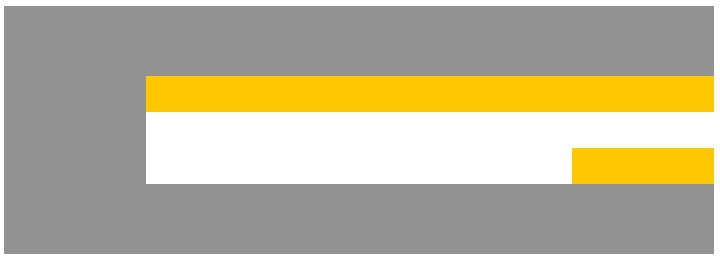
\includegraphics[width=\linewidth]{fig/cant_single_side.jpg}
	    	\caption{This is the second figure}
            \label{fig:cant_single_side}
		\end{figure}
	\end{minipage}
\end{minipage}

\subsection{Actuation}
\label{sec:actuation}
There are four different actuation principles which can be used for a mechanical micro-switch design:
\begin{itemize}
  \item Electrostatic
  \item Piezoelectric
  \item Electromagnetic
  \item Thermal
\end{itemize}

Thermal actuators are not fast enough for micro-switch applications. 
Also they have the highest power consumption of all the methods.

Electromagnetic actuators require either a permanent magnetic material or an electromagnet design to work.
The material choices are therefore difficult and also the footprint would be rather big compared to the other methods.

Piezoelectric actuators represent the method with the lowest power consumption.
But compared to electrostatic actuators they are way more complex to fabricate and material choices represent a challenge.\cite{klaasse2002piezoelectric}

Therefore our choice fell on an electrostatic actuator.
They are very simple from a fabrication point of view, allow low power consumption and offer a fast actuation time.

\subsection{Basic Concepts}
\label{sec:basic_concepts}

Our switch design is based on a beam cantilever, so we start with the deflection of a clamped beam with a force applied at an arbitrary point along the beam (\ref{eq:beam_deflection}).

\begin{equation}
    \delta(x) = \begin{cases} \frac{Fx^2}{6EI_z} \cdot (3a-x) & \mbox{for } 0 < x < a \\
                              \frac{Fa^2}{6EI_z} \cdot (3x-a) & \mbox{for } a < x < l
                \end{cases}
    \label{eq:beam_deflection}
\end{equation}


With the area moment of inertia defined as such:
\begin{equation}
	I_z = \frac{wt^3}{12}
	\label{eq:area_moment_of_inertia}
\end{equation}

and the distance $a$ like it is shown in Figure~\ref{fig:cantilever_beam}.

\begin{figure}[h]
	\centering
	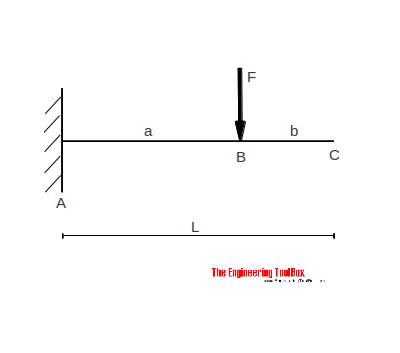
\includegraphics[width=8cm]{fig/cantilever_beam_single_load.png}
    \caption{Clamped beam with a single load.}
\label{fig:cantilever_beam}
\end{figure}

\subsubsection{Resonance frequency}
In order to estimate the time it takes to flip the switch, we calculate the \emph{resonance frequency} of the beam.
We can simplify the cantilever as a harmonic oscillator (mass-spring).
In that case we calculate the resonance frequency using equation (\ref{eq:resonance_frequency}).

\begin{equation}
	\omega_0 = \sqrt{\frac{k}{m_{eff}}}
	\label{eq:resonance_frequency}
\end{equation}

We need to calculate the spring constant $k$ and the effective mass $m_{eff}$ of the beam.
From (\ref{eq:beam_deflection}) we can conclude (\ref{eq:spring_constant}) for the spring constant.

\begin{equation}
	k = \frac{F}{\delta} = \frac{6EI_z}{a^2(3l-a)}
	\label{eq:spring_constant}
\end{equation}

Equation (\ref{eq:effective_mass}) defines the effective mass~\cite{wong2011theoretical}.

\begin{equation}
	m_{eff} = \rho A \int_0^l{\left[\frac{\delta(x)}{\delta(l)_{max}}\right]^2dx}
	\label{eq:effective_mass}
\end{equation}

If we evaluate (\ref{eq:effective_mass}) for a beam with the force applied at the extremity, we get $m_{eff} = 33/140 m$.
When we apply the force at an arbitrary position $a$, the expression becomes $m_{eff} = \frac{6l^2-4al+a^2}{12l^2-4al} m$.
If we choose a value for $a$ more or less close to $l$, we can just use $33/140m$ for simplicity.


\subsubsection{Electrostatic force}
Note: Distance smaller than surface, neglect fringes because of aspect ratio
Equation (\ref{eq:electrostatic_force}) gives the electrostatic force between two metal plates.
One notes that this is neglecting any \emph{fringe effects}.
We can do that when the distance between the plates is much smaller than the side lengths of the plates.

\begin{equation}
	F_{ES} = \frac{\varepsilon AV^2}{2d^2}
	\label{eq:electrostatic_force}
\end{equation}

\subsubsection{Switch resistance}
\begin{equation}
	R = \rho_{el}\frac{l}{wt}
	\label{eq:resistance}
\end{equation}

\subsubsection{Actuator pad capacitance}
The actuator forms a \emph{capacitor}, which we have to charge when we want to operate the switch.
This charging takes time we have to make sure that it isn't a limiting factor.

Equation (\ref{eq:plate_capacitor}) gives the \emph{capacitance} of the actuator.

\begin{equation}
	C = \frac{\varepsilon A}{d}
	\label{eq:plate_capacitor}
\end{equation}

We then get the time constant $\tau$ in equation (\ref{eq:rc_time_constant}).

\begin{equation}
    \tau = RC
    \label{eq:rc_time_constant}
\end{equation}

With $R$ being the resistance of the circuit charging the capacitor.

\subsubsection{Thermal analysis}

We neglect any thin-film effects and there are no currents expected to be high enough to heat the mechanism up to a point where it starts to matter.

\subsection{Analysis}
\label{sec:analysis}
- Actuation point vs contact point placement
- Area contact
- Area actuator
- Beam cross section
- Material
